La metodología a utilizar es la metodología de desarrollo ágil Melé\footnote{Desde la Séptima Edición del libro ``Ingeniería del software. Un enfoque practico.'' del Ph.D. Roger S. Pressman, es llamado Scrum. }~\cite{7}.

En la \textbf{Figura~\ref{fig: procesoMele}} se puede observar que Melé tiene un conjunto de \emph{``patrones de proceso de software''} los cuales definen un conjunto de actividades de desarrollo:

\begin{itemize}
    

    \item   \begin{description}
                \item[Sprint:] proceso por el cual se requiere satisfacer un requisito definido en los retrasos en un periodo predefinido (usualmente es de 30 días). Cuando se comienza un Sprint, no se pueden agregar nuevos cambios. Por lo tanto, esto permite trabajar en un ambiente enfocado a corto plazo, pero estable.
            \end{description}

    

    
\end{itemize}

\begin{figure}[h!]
    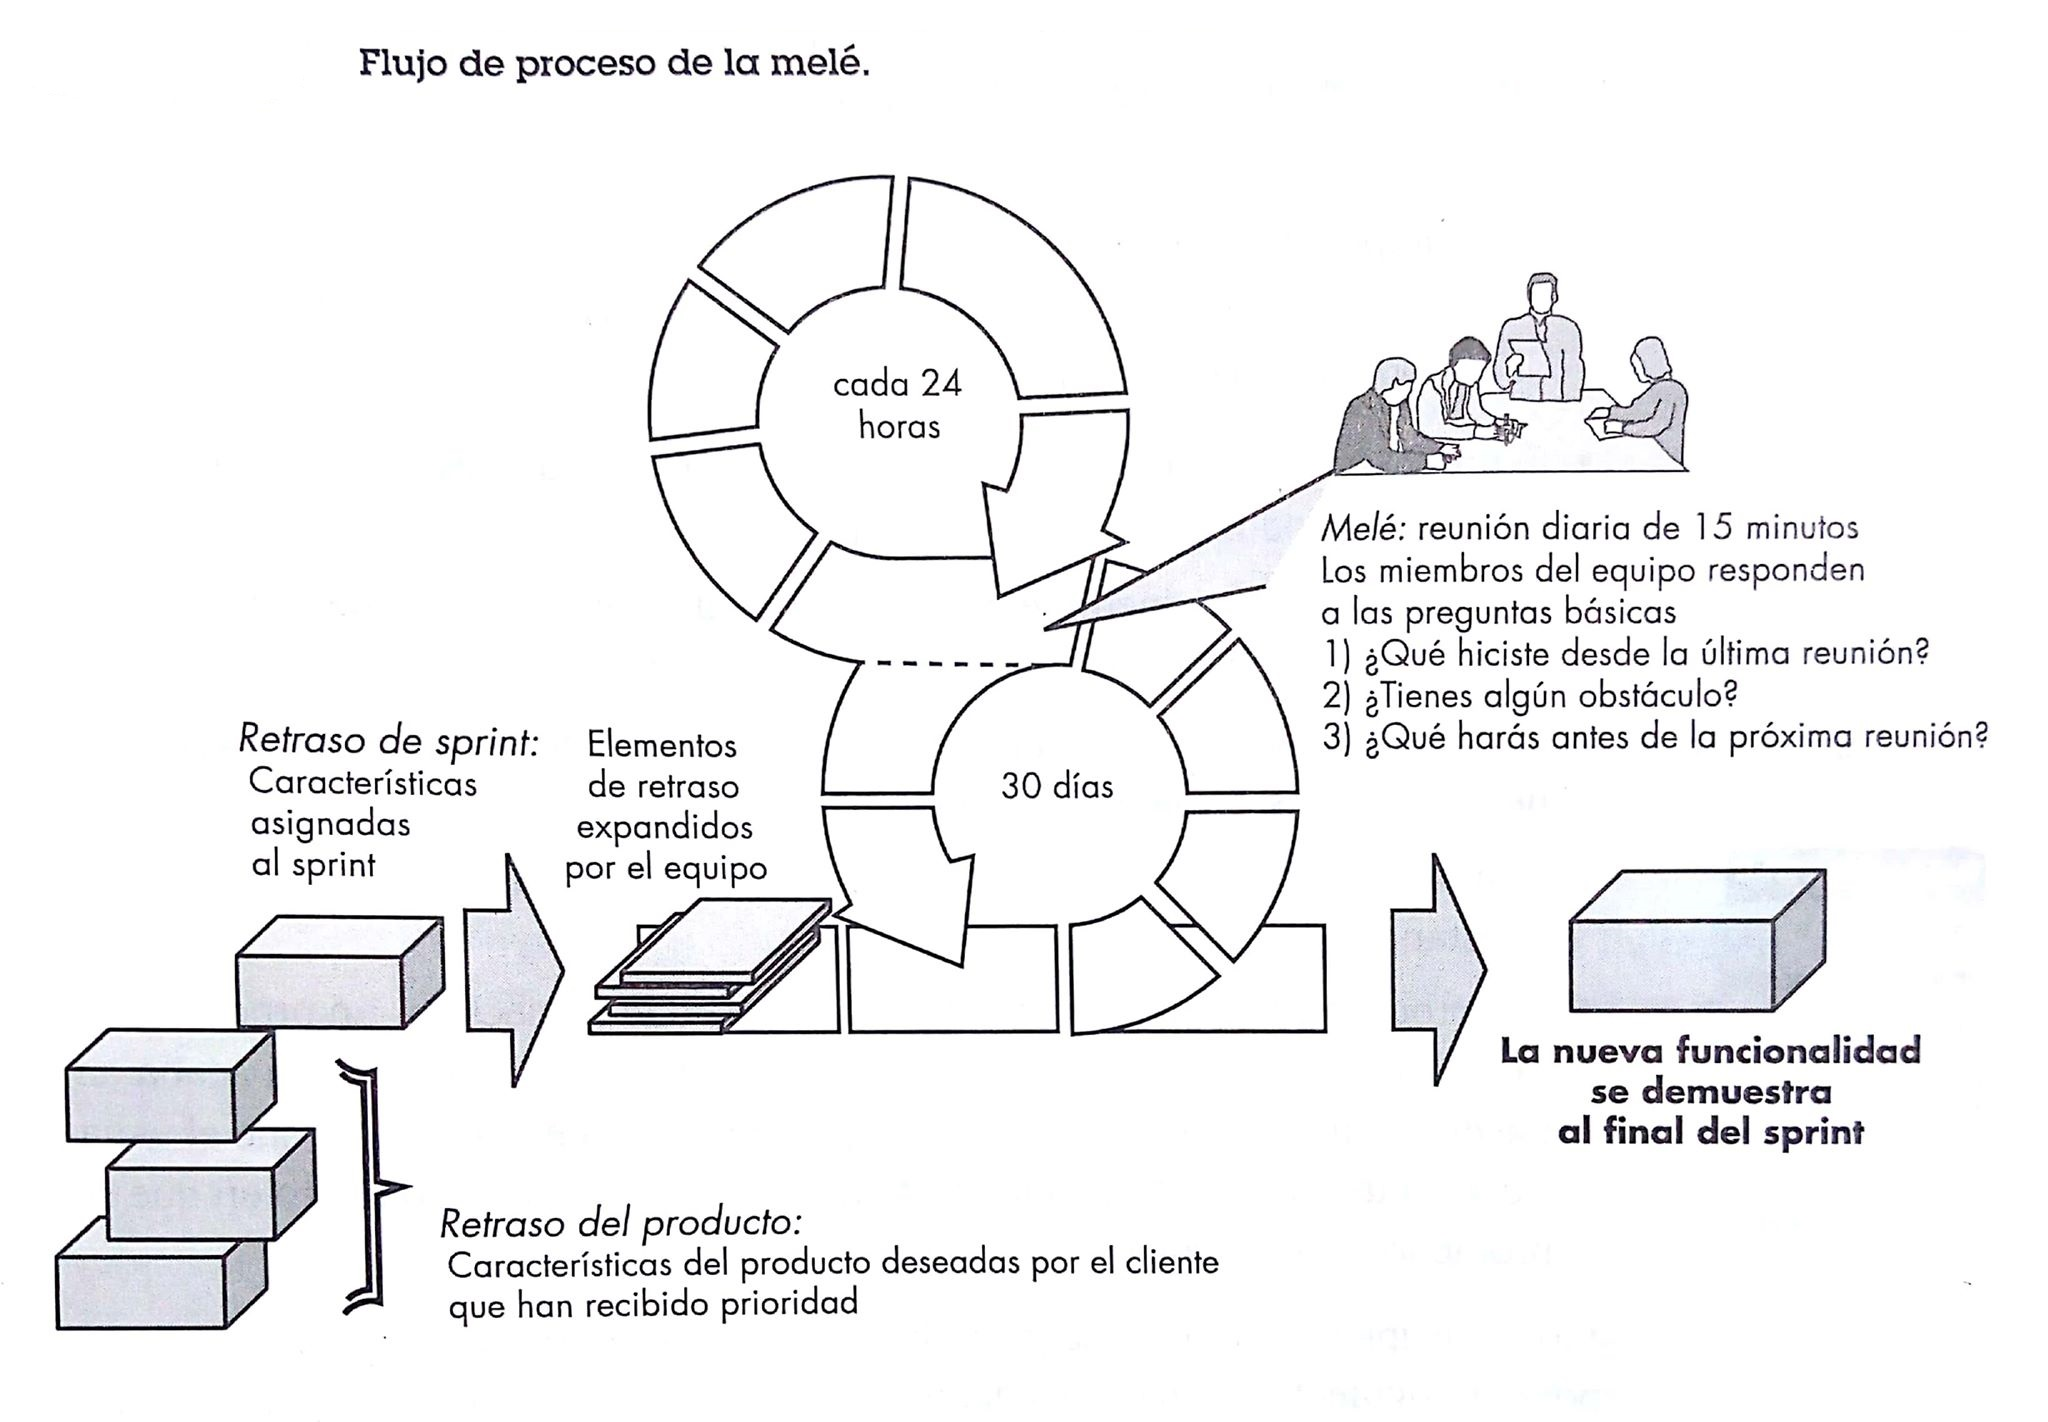
\includegraphics[width=\textwidth]{Imagenes/mele.jpg}
    \caption{\label{fig: procesoMele} Proceso de metodología Melé.}
\end{figure}
